\section{Teste de gráficos}
\subsection{Árvores}

\usetikzlibrary{trees}

%escolher o melhor pacote
%inserir o nome do nó num círculo
%inserir duas arvores lado a lado
%inserir titulo para a arvore
%inserir setas a conectares dduas subarvores
%colocar rectangulo na subarvore da mutacao/cruzamento

\begin{figure}[H]
	\centering
	\begin{minipage}{.33\linewidth}
		\centering
		\begin{forest}
			%for tree={circle, draw}
			[{Pai 1}, baseline, for children={no edge}
			[$+$,circle,draw,
				[$*$,circle,draw
					[$x_1$,circle,draw]
					[$x_2$,circle,draw]
				]
				[,phantom]
				[$-$,name=cppai1,circle,draw,tikz={\node [draw,red,fit to tree,dashed] {};}
					[$x_2$,circle,draw,name=cima]
					[$x_1$,circle,draw]
				]
			]
			]
		\end{forest}
	\end{minipage}
	\hspace*{5em}
	\begin{minipage}{.33\linewidth}
		\centering
		\begin{forest}
			%for tree={circle, draw}
			[{Filho 1}, baseline, for children={no edge}
			[$+$,circle,draw,
				[$*$,circle,draw
					[$x_1$,circle,draw]
					[$x_2$,circle,draw]
				]
				[,phantom]
				[$*$,circle,draw,tikz={\node [draw,red,fit to tree,dashed] {};}
					[$x_1$,circle,draw,name=baixo]
					[$x_1$,circle,draw]
				]
			]
			]
			\draw[-,solid] (baixo) to [out=south west,in=south] (cima);
		\end{forest}
	\end{minipage}
	\caption{Exemplo de cruzamento de subárvore}
\end{figure}


\begin{figure}[H]
	\centering
    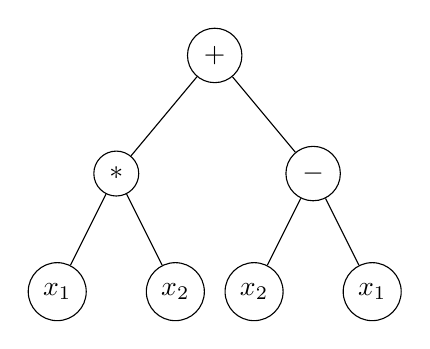
\begin{tikzpicture}[auto, every node/.style={circle,draw}, remember picture] 
    	\tikzstyle{level 1}=[sibling distance=2.5cm] 
    	\tikzstyle{level 2}=[sibling distance=1.5cm] 
    	\node (a1){$+$}
	    	child{ 
	    		node (cp11) {$*$}
	    		child{node (cp111) {$x_1$}} 
	    		child{node (cp112) {$x_2$}}
	    	}
	    	child{ 
	    		node (cp12) {$-$}
	    		child{node (cp121) {$x_2$}} 
	    		child{node (cp122) {$x_1$}}
	    	}
	    ;
	\end{tikzpicture}
    \begin{tikzpicture}[auto, every node/.style={circle,draw}, shift={(23.2cm,-1cm)},remember picture, overlay] 
    	\tikzstyle{level 1}=[sibling distance=2.5cm] 
    	\tikzstyle{level 2}=[sibling distance=1.5cm] 
    	\node (a2){$+$}
	    	child{ 
	    		node (cp21) {$*$} 
	    		child{node (cp211) {$x_1$}} 
	    		child{node (cp212) {$x_2$}}
	    	}
	    	child{ 
	    		node (cp22) {$*$}
	    		child{node (cp221) {$x_1$}} 
	    		child{node (cp222) {$x_1$}}
	    	}
	    ;
	    \draw[color=blue,<->] (cp221)  edge[out=0, in=0] (cp11);
    \end{tikzpicture}
    \caption{Exemplo de cruzamento de subárvore}
\end{figure}

OUTRO EXEMPLO